\chapter{Platform}

\begin{figure}[H]
	\centering
	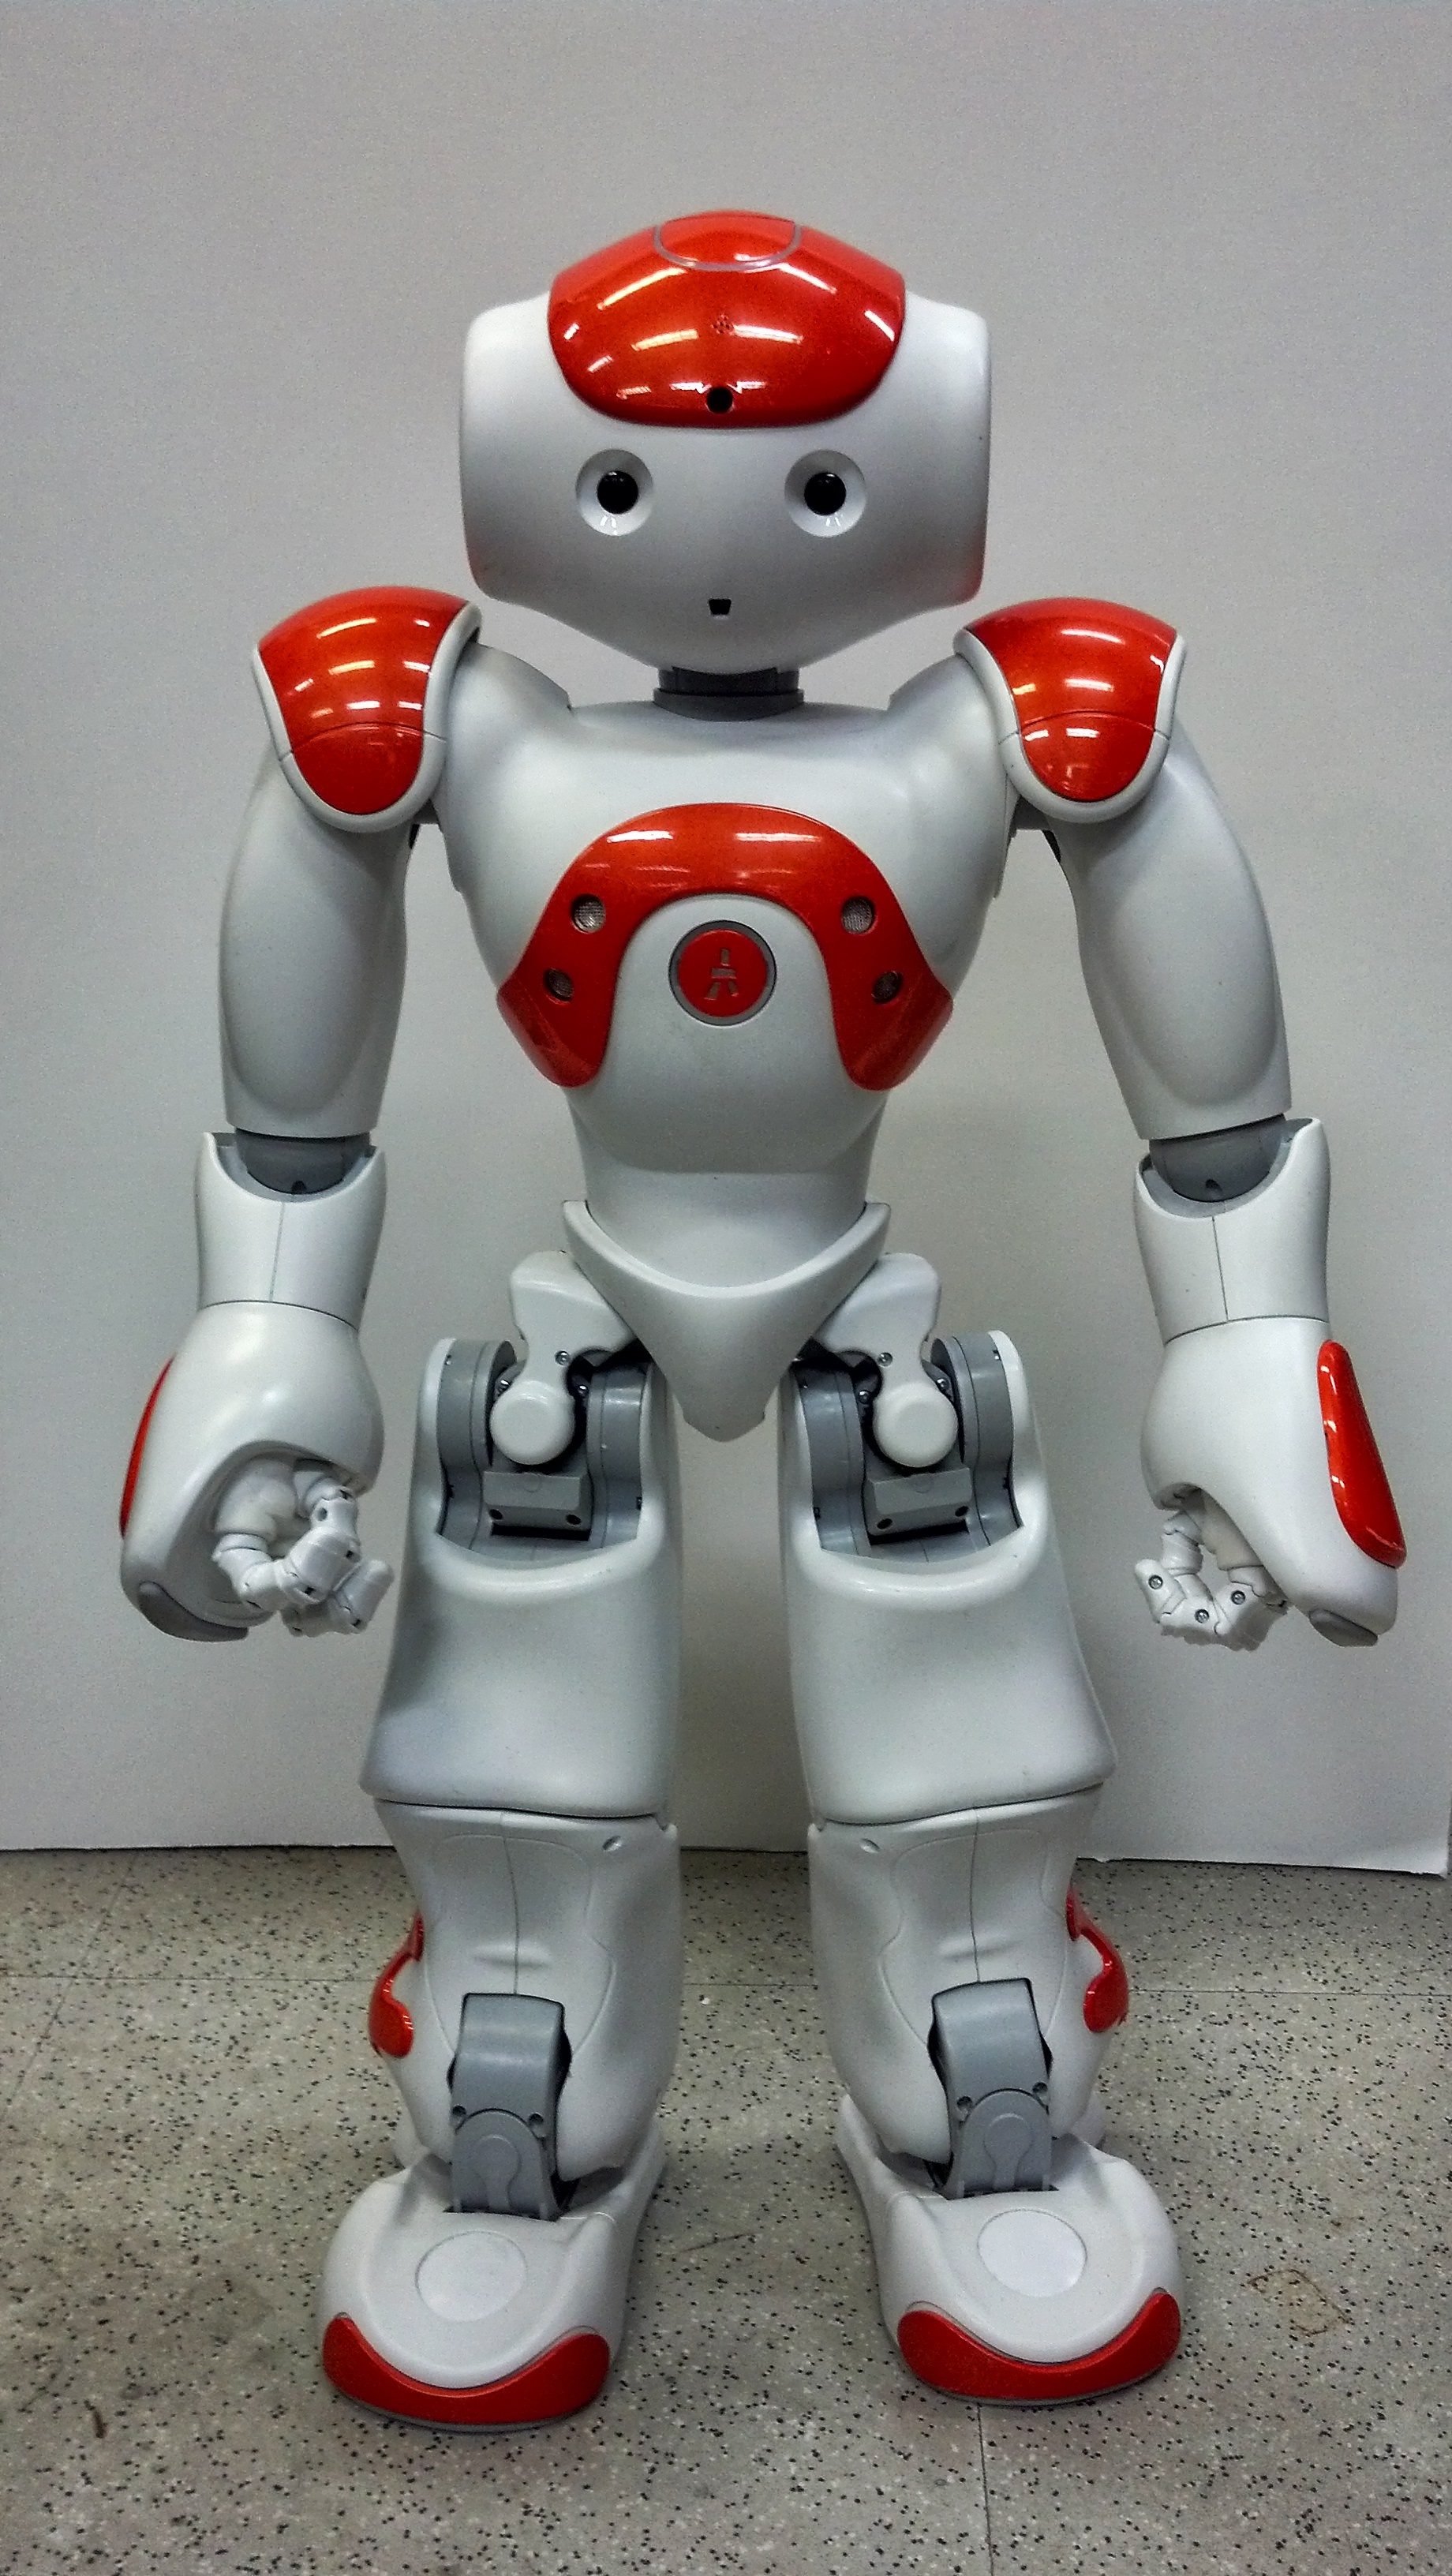
\includegraphics[width=0.35\textwidth]{nao1.jpg}
	\caption
	{Nao robot at Control/Robotics Research Lab}
	\label{fig:nao1}
\end{figure}

The platform utilized on this project was the Nao humanoid experimental robotic platform by Aldebaran Robotics. It is a 25 degree-of-freedom humanoid mobile manipulator with two HD cameras, two ultrasonic distance sensors, four microphones, one three-axis accelerometer, two one-axis gyroscopes, and four force sensors in each foot. The platform is programmed using a framework called NAOqi allowing development using various languages including C++ and Python. 

\section{Distance Sensors}
Two ultrasonic sensors in the chest allowed for distance measurements to occlusions. The transmitters are mounted at an angle of 20 degrees from the forward direction of the Nao and the receivers are mounted at 25 degrees. They have a 60 degree viewing angle with a detection range between 0.25 and 2.55 meters with a 1 cm resolution.

\begin{figure}[h]
	\centering
	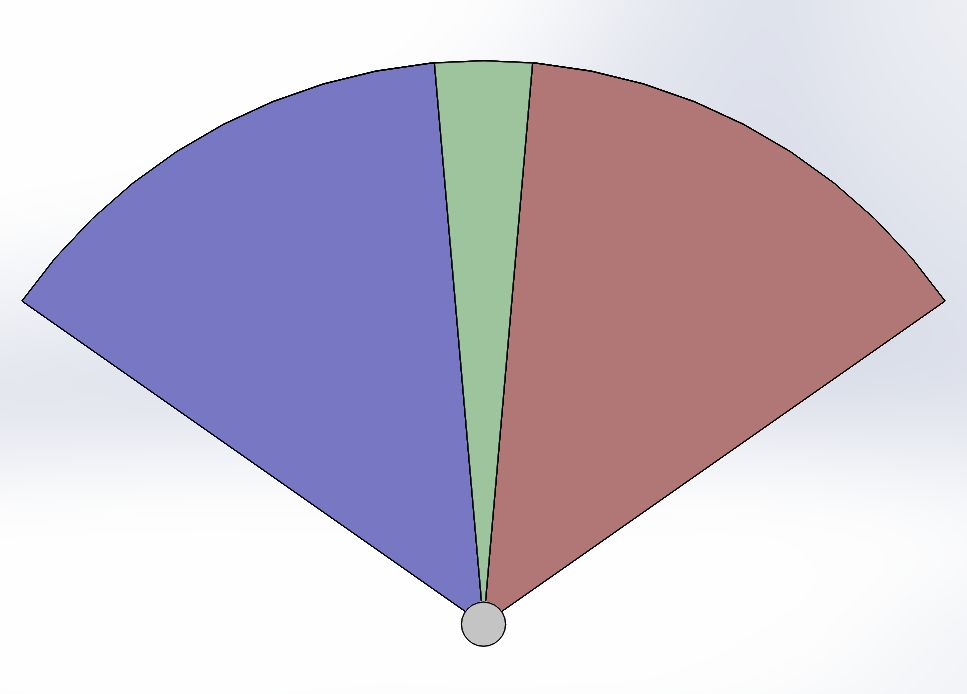
\includegraphics[width=0.35\textwidth]{sonar1.jpg}
	\caption
	[Nao sonar cones.]
	{Nao sonar cones. The left cone is shown in blue and the right cone is shown in red. The green cone shows the overlap between the two.}
	\label{fig:sonar1}
\end{figure}

As shown in Figure \ref{fig:sonar1} the regions covered by the two ultrasonic sensors overlap. As the sensors do not report the angular position of the occlusion within the cone, uncertainty about the location of detected objects is high as they could be anywhere within the sonar cone.

The distance measurements also suffered from multipath returns and specular reflections which caused the robot to read incorrect distances at certain angles. For example, at times when the Nao was oriented toward a wall at an obtuse angle, the right distance sensor, which was closer to the wall, would read a distance much larger than that of the left sensor, causing the robot to gravitate into the wall. An example of the problem can be seen in Figure \ref{fig:sonar2}.

\begin{figure}[h]
	\centering
	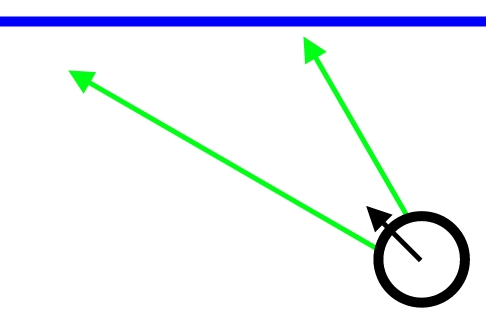
\includegraphics[width=0.35\textwidth]{sonar2.jpg}
	\caption
	[Distance measurement error at obtuse angles.]
	{Distance measurement error at obtuse angles. In the figure, the black circle represents the Nao in the plane, 
		while black arrow represents the current heading. The blue line represents a wall and the green arrows indicate
		the direction the sonars are pointing. When in positions similar to this the right sensor would report a distance
		greater than the left sensor, even though the right sensor is closer to the wall.}
	\label{fig:sonar2}
\end{figure}

At times, the source of erroneous sensor measurements stemmed from the material that the occlusion was made from. It was found that if the material was too soft the distance reported to it would be larger, or at times, not be seen. Harder materials seemed to correct for this. Soft materials were items like plastic trash cans. Metal trash cans responded more reliably.
A brief overview about various issues with sonar can be read about here \cite{sonar_issues1}.

\section{Programming}
For this project, code was not compiled on the Nao itself but rather on an external computer and commands were send to the Nao via a Wi-Fi network that both the Nao and the external computer were connected to. After setting up the build system qiBuild 
\cite{qiBuild_tutorial1} on the external computer, a new project is built using qiBuild and then edited and complied using Visual Studio 2008. Once built, the executable from the project is run from the command line with the IP address of the Nao as an argument and the Nao responds. Any print statements are seen on the command line.

The NAOqi framework uses the concept of proxies in order to access sensor data or send movement commands. Proxies are objects where data is accessed, stored, or sent. They are proxy to where these items are actually used or accessed, which are the Nao's memory, referenced using memory keys \cite{memory1}. For example, the memory keys for accessing the distance measurements for the sonar are:

\begin{lstlisting}[frame=single]
	Device/SubDeviceList/US/Right/Sensor/Value
	Device/SubDeviceList/US/Left/Sensor/Value
\end{lstlisting}

whose reference can be seen here \cite{sonar_ref1}.

The motion API used in this project was 

\begin{lstlisting}[frame=single]  
void ALMotionProxy::setWalkTargetVelocity(const float& x, const float& y, const float& theta, const float& frequency)
\end{lstlisting}

It takes three different velocity commands, forward, lateral, and angular, in terms of fraction of maximum step length and step frequency. The maximum step length is 8 cm forward, 16 cm laterally, and 0.523 radians angularly. The maximum step frequency is 2.381 Hz. Due to a stability controller in the built-in gaiting algorithm for the Nao, it takes 0.8 seconds for the robot to react to new commands. At maximum step frequency, this equates to about 2 steps. \cite{naodoc_motion1}

Talk about built in red ball tracking for head that returns range and bearing estimates of a red ball 6 cm in diameter.

